\documentclass[11pt]{article}
\usepackage[scaled=0.92]{helvet}
\usepackage{geometry}
\geometry{letterpaper,tmargin=1in,bmargin=1in,lmargin=1in,rmargin=1in}
\usepackage[parfill]{parskip} % Activate to begin paragraphs with an empty line rather than an indent %\usepackage{graphicx}
\usepackage{amsmath,amssymb, mathrsfs,  mathtools, dsfont}
\usepackage{tabularx}
\usepackage[font=footnotesize,labelfont=bf]{caption}
\usepackage{graphicx}
\usepackage{xcolor}
%\usepackage[linkbordercolor ={1 1 1} ]{hyperref}
%\usepackage[sf]{titlesec}
\usepackage{natbib}
\usepackage{../../Tianpei_Report}

%\usepackage{appendix}
%\usepackage{algorithm}
%\usepackage{algorithmic}

%\renewcommand{\algorithmicrequire}{\textbf{Input:}}
%\renewcommand{\algorithmicensure}{\textbf{Output:}}



\begin{document}
\title{Lecture 2: Banach Space}
\author{ Tianpei Xie}
\date{ Nov. 19th., 2022 }
\maketitle
\tableofcontents
\newpage
\section{Normed Linear Space}
\begin{itemize}
\item \begin{definition}
A \emph{\textbf{metric space}} is a set $M$ and a real-valued function $d(\cdot , \cdot): M \times M \rightarrow \bR$  which satisfies:
\begin{enumerate}
\item (\emph{\textbf{Non-Negativity}}) $d(x, y) \ge 0$
\item (\emph{\textbf{Definiteness}}) $d(x, y) = 0$ if and only if $x = y$
\item (\emph{\textbf{Symmetric}}) $d(x, y) = d(y, x)$
\item (\emph{\textbf{Triangle Inequality}}) $d(x, z) \le d(x, y) + d(y, z)$
\end{enumerate} The function $d$ is called a \underline{\emph{\textbf{metric}}} on $M$. The metric space $M$ equipped with metric $d$ is denoted as $(M, d)$.
\end{definition}

\item \begin{remark}
Note that the definition of a \emph{metric space} is only about the \emph{\textbf{topology}} of the space. In the field of functional analysis,  we are mostly concerned about \emph{\textbf{the vector space}}, i.e. a space that equipped with algebraic operations such as vector addition and  scalar multiplications. In order to make the \emph{\textbf{metric}\textbf{ topological structure}} \emph{\textbf{compatible}} with \emph{\textbf{the algebraic structure} of \textbf{vector space}}, we need to introduce additional function such as the \emph{\textbf{norm}}.
\end{remark}

\item \begin{definition} (\emph{\textbf{Normed Linear Space}})\\
A \underline{\emph{\textbf{normed linear space}}} is a vector space, $V$, over $\bR$ (or $\bC$) and a function, $\norm{\cdot}{}: V \rightarrow \bR$ which satisfies:
\begin{enumerate}
\item (\emph{\textbf{Non-Negativity}}): $\norm{v}{} \ge 0$ for all $v$ in $V$;
\item (\emph{\textbf{Positive Definiteness}}): $\norm{v}{} = 0$ if and only if $v = 0$;
\item (\emph{\textbf{Absolute Homogeneity}}) $\norm{\alpha v}{} = \abs{\alpha}\norm{v}{}$ for all $v$ in $V$ and $\alpha$ in $\bR$ (or $\bC$)
\item (\emph{\textbf{Subadditivity / Triangle Inequality}}) $\norm{v + w}{}\le \norm{v}{} + \norm{w}{}$ for all $v$ and $w$ in $V$
\end{enumerate}
We denote the normed linear space as $(V, \norm{\cdot}{})$.
\end{definition}

\item \begin{remark}
If the function $p: V \rightarrow \bR$ only satisfies the condition 1, 3 and 4 (without \emph{positive definiteness}), it is called a \underline{\emph{\textbf{semi-norm}}}. The 1. \emph{non-negativity} condition can be derived by the 3. \emph{homogeneity} and 4. \emph{subadditivity} conditions. 
\end{remark}

\item \begin{remark}
\emph{A normed linear space} $(V, \norm{\cdot}{})$ is a \emph{\textbf{metric space}} with \emph{induced metric }
\begin{align*}
d(x, y) = \norm{x - y}{}, \quad \text{for all } x, y \in V
\end{align*}
\end{remark}



\item \begin{definition} (\emph{\textbf{Bounded Linear Operator}})\\
A \underline{\emph{\textbf{bounded linear transformation}}} (or \emph{\textbf{bounded operator}}) is a mapping $T: (X, \norm{\cdot}{X}) \rightarrow (Y, \norm{\cdot}{Y})$ from a normed linear space $X$ to a normed linear space $Y$ that satisfies 
\begin{enumerate}
\item (\emph{\textbf{Linearity}}) $T(\alpha x + \beta y) = \alpha T(x) + \beta T(y)$ for all $x, y \in X$, $\alpha, \beta \in \bR$ or $\bC$
\item (\emph{\textbf{Boundedness}}) $\norm{Tx}{Y} \le C\,\norm{x}{X}$ for small $C \ge 0$.
\end{enumerate} The smallest such $C$ is called \underline{\emph{the \textbf{norm} of $T$}}, written $\norm{T}{}$ or $\norm{T}{X, Y}$. Thus
\begin{align*}
\norm{T}{} &:= \sup_{\norm{x}{X} = 1 }\norm{Tx}{Y}
\end{align*}
\end{definition}

\item \begin{remark}
\emph{A linear operator} $T$ is a \emph{\textbf{homomorphism} of a vector space (its domain) into another vector space}, that is, \emph{$T$ \textbf{preserves} the \textbf{two operations} of vector space}.
\end{remark}

\item \begin{proposition} \citep{reed1980methods, kreyszig1989introductory}\\
Let $T$ be a linear transformation between two \textbf{normed linear spaces}. The following are \textbf{equivalent}:
\begin{enumerate}
\item $T$ is \textbf{continuous} at \textbf{one} point.
\item $T$ is \textbf{continuous} at \textbf{all} points.
\item $T$ is \textbf{bounded}.
\end{enumerate}
\end{proposition}

\item \begin{definition}
A normed linear space $(V, \norm{\cdot}{})$  is \underline{\emph{\textbf{complete}}} if it is \emph{complete} as a \emph{metric space} in \emph{the induced metric}.
\end{definition}

\item \begin{theorem} (\textbf{The B.L.T. Theorem}) \citep{reed1980methods}\\
Suppose $T$ is a bounded linear transformation from a normed linear space $(V_1, \norm{\cdot}{1})$ to a \textbf{complete} normed linear space $(V_2, \norm{\cdot}{2})$. Then $T$ can be \textbf{uniquely extended} to a bounded linear transformation (with the same bound), $\widetilde{T}$, from the \textbf{completion} of $V_1$ to $(V_2, \norm{\cdot}{2})$.
\end{theorem}
\end{itemize}

\section{Banach Space}
\subsection{Definition and Examples}
\begin{itemize}
\item \begin{definition}
A \emph{\textbf{complete}} \emph{normed linear space} is called a \underline{\emph{\textbf{Banach space}}}.
\end{definition}

\item \begin{example} ($\cC(X)$ and its subspace $\cC_{\bR}(X)$)\\
Let $\cC(X)$ be the set of all \emph{complex-valued \textbf{continuous functions}} on $X$ and $\cC_{\bR}(X) \subseteq \cC(X)$ be the set of all \emph{\textbf{real-valued continuous functions}} on $X$. Also define $\cC^{b}(X)$ as the set of all \emph{complex-valued \textbf{bounded continuous functions}} on $X$. When $X$ is \emph{\textbf{a compact space}}, $\cC^{b}(X) = \cC(X)$.  Define the norm as 
\begin{align*}
\norm{f}{\infty} &= \sup_{x\in X}\abs{f(x)}.
\end{align*} Then for \underline{\emph{\textbf{compact Hausdorff space}} $X$}, \underline{$\cC(X)$ is a \emph{(complex) \textbf{Banach space}}} and $\cC(X)$ is \emph{\textbf{a (real) Banach space}}.
\end{example}


\item \begin{example} (\emph{\textbf{$L^{\infty}(\bR)$ and its subspace $\cC^{0}(\bR)$}})\\
Let $L^{\infty}(\bR)$ be the set of (\emph{equivalence classes of}) \emph{complex-valued measurable functions} on $\bR$ such that $\abs{f(x)}\le M$ a.e. with respect to Lebesgue measure for some $M < \infty$ ($f = g$ means $f(x) = g(x)$ a.e.). Let $\norm{f}{\infty}$ be \emph{\textbf{the smallest such $M$}}. \underline{$L^{\infty}(\bR)$ is a \emph{\textbf{Banach space}}} with norm $\norm{\cdot}{\infty}$. 

\underline{\emph{The \textbf{bounded continuous functions}} $\cC^{0}(\bR)$ is a \emph{\textbf{subspace}} of $L^{\infty}(\bR)$}  and restricted to $\cC^{0}(\bR)$ the $\norm{\cdot}{\infty}$-norm is just the usual \emph{\textbf{supremum norm}} under which $\cC^{0}(\bR)$  is \underline{\emph{\textbf{complete}}} (since \emph{the uniform limit of continuous functions is continuous} See proof in chapter 1.). Thus, \emph{\textbf{$\cC^{0}(\bR)$ is a closed subspace of $L^{\infty}(\bR)$ }}.

Consider the set $\kappa(\bR)$ of \emph{\textbf{continuous functions} with \textbf{compact support}}, that is, the continuous functions that \emph{vanish outside of some closed interval}.  $\kappa(\bR)$  is a \emph{\textbf{normed linear space}} under $\norm{\cdot}{\infty}$; but \emph{is \textbf{not complete}}, The \emph{\textbf{completion}} of $\kappa(\bR)$ is \emph{\textbf{not all} of $\cC^{0}(\bR)$}; for example, if $f$ is the function which is identically equal to one, then I \emph{cannot be approximated by a function in $\kappa(\bR)$} since $\norm{f - g}{\infty} \ge 1$ for all $g \in \kappa(\bR)$. The \emph{\textbf{completion}} of $\kappa(\bR)$ is just $\cC_{\infty}(\bR)$, \emph{the continuous functions which \textbf{approach zero} at $\infty$}. 

Some of the most powerful theorems in functional analysis (\emph{Riesz-Markov}, \emph{Stone-Weierstrass}) are generalizations of properties of $\cC^{0}(\bR)$. \qed
\end{example}

\item \begin{example} (\emph{\textbf{$L^{p}$ spaces}})\\
Let $(X, \mu)$ be a measure space and $p\ge 1$. We denote by $L^{p}(X, \mu)$ \emph{\textbf{the set of equivalence classes}} of measurable functions which satisfy:
\begin{align*}
\norm{f}{p} &:= \paren{\int_{X}\abs{f(x)}^p d\mu(x)}^{\frac{1}{p}} < \infty
\end{align*} Two functions are \emph{equivalent} if they differ only on \emph{a set of measure zero}.

The following theorem collects many of the standard facts about $L^{p}$ spaces.
\begin{theorem}
Let $1 \le p < \infty$, then
\begin{enumerate}
\item \underline{(\textbf{The Minkowski Inequality})}: If $f, g \in L^{p}(X, \mu)$, then
\begin{align*}
\norm{f +g}{p} &\le \norm{f}{p} + \norm{g}{p}
\end{align*}
\item  \underline{(\textbf{Riesz-Fisher})}:  $L^{p}(X, \mu)$ is \textbf{complete}.
\item \underline{(\textbf{The H\"older Inequality})} Let $p, q$, and $r$ be positive numbers satisfying
$p, q, r \ge 1$ and $p^{-1} +q^{-1} = r^{-1}$. Suppose  $f \in L^{p}(X, \mu)$, $g \in L^{q}(X, \mu)$. Then
$fg \in L^{r}(X, \mu)$ and
\begin{align*}
\norm{fg}{r} &\le \norm{f}{p}\,\norm{g}{q}
\end{align*}
\end{enumerate}
\end{theorem}

\begin{remark}
\emph{The Minkowski inequality} shows that $L^{p}(X, \mu)$ is a vector space and $\norm{\cdot}{p}$ satisfies the triangle inequality. This together with \emph{Riesz-Fisher theorem} shows that \emph{\textbf{$L^{p}(X, \mu)$ is a Banach space}}.
\end{remark}
\end{example}



\item \begin{example}(\emph{\textbf{Sequence Spaces}})\\
There is a nice class of spaces which is easy to describe and which we will often use to illustrate various concepts.
In the following definitions,
\begin{align*}
a &:= (a_n)_{n=1}^{\infty}
\end{align*} always denotes a sequence of complex numbers.
\begin{align*}
\ell^{\infty} &:= \set{a: \norm{a}{\infty}:= \sup_{n}\abs{a_n} < \infty }\\
c_{0} &:= \set{a: \lim\limits_{n\rightarrow \infty}a_n = 0}\\
\ell^{p} &:= \set{a: \norm{a}{p}:= \paren{\sum_{n=1}^{\infty}\abs{a_n}^{p}}^{\frac{1}{p}} < \infty }\\
s &:= \set{a:  \lim\limits_{n\rightarrow \infty}n^{p}a_{n}= 0 \text{ \emph{for all positive integers} }p}\\
f &:=  \set{a: a_{n} = 0\text{ \emph{for all but a finite number of} }n}
\end{align*} It is clear that as sets $f \subseteq s \subseteq \ell^{p} \subseteq c_{0} \subseteq \ell^{\infty}$.

\underline{\emph{\textbf{The spaces $\ell^{\infty}$ and $c_{0}$ are Banach spaces with the $\norm{\cdot}{\infty}$ norm}}}; \emph{\textbf{\underline{$\ell^{p}$ is a Banach space} with the $\norm{\cdot}{p}$ norm}} (note that $\ell^{p}= L^{p}(\bR, \mu)$ where $\mu$ is the measure with \emph{mass one at each positive integer} and \emph{zero} everywhere else). It will turn out that \emph{\textbf{$s$ is a Frechet space}}. 

One of the reasons that these spaces are easy to handle is that \emph{\underline{$f$ is \textbf{dense} in $\ell^{p}$} (in $\norm{\cdot}{p}$; $p < \infty$} and \emph{\textbf{\underline{$f$ is dense in $c_{0}$} (in the $\norm{\cdot}{\infty}$ norm)}}. Actually, the set of elements of $f$ with only \emph{rational entries} is also \textbf{dense} in $\ell^{p}$ and $c_{0}$. Since this set is \emph{\textbf{countable}}, $\ell^{p}$ and $c_{0}$ are \emph{\textbf{separable}}. \emph{\textbf{$\ell^{\infty}$ is not separable}}.
\end{example}

\item \begin{example}(\emph{\textbf{The Bounded Operators}})\\
In above we defined the concept of a \emph{bounded linear transformation} or \emph{bounded operator} from one normed linear space, $X$, to another $Y$; we will denote \emph{the set of all bounded linear operators from $X$ to $Y$ by $\cL(X, Y)$}. We can introduce a \emph{norm} on  $\cL(X, Y)$ by defining
\begin{align*}
\norm{A}{} &:= \sup_{x \neq 0, \, x \in X} \frac{\norm{Ax}{Y}}{\norm{x}{X}}.
\end{align*}
This norm is often called \underline{\emph{\textbf{the operator norm}}}.

We have the following proposition
\begin{proposition} \label{prop: bounded_operator_banach}
If $Y$ is \textbf{complete}, $\cL(X, Y)$ is a \textbf{Banach space}.
\end{proposition}
\end{example}

\item \begin{example} (\emph{\textbf{Hilbert Space}})\\
All \emph{\textbf{Hilbert spaces}} $(\cH, \inn{\cdot}{\cdot})$ are \textbf{\emph{Banach spaces}} with \emph{induced norm} as
\begin{align*}
\norm{x}{} &= \paren{\inn{x}{x}}^{\frac{1}{2}}.
\end{align*} 
\end{example}
\end{itemize}

\subsection{Isomorphism and Equivalence of Norms}
\begin{itemize}
\item \begin{definition} (\emph{\textbf{Absolutely Summable}})\\
A sequence of elements $(x_n)_{n=1}^{\infty}$ in a \emph{normed linear space} $X$ is called \emph{\textbf{absolutely summable}} $\sum_{n=1}^{\infty}\norm{x_n}{} < \infty$. It is called \emph{\textbf{summable}} if $\sum_{n=1}^{N}x_n$ \emph{converges} as $N \rightarrow\infty$ to an $x \in X$.
\end{definition}

\item \begin{proposition} (\textbf{Criterion of Completeness for Normed Linear Space}) \citep{reed1980methods} \\
A normed linear space is \textbf{complete} if and only if every \textbf{absolutely summable} sequence is \textbf{summable}.
\end{proposition}

\item \begin{definition} (\emph{\textbf{Isomorphism between Normed Linear Spaces}})\\
A \textit{\textbf{bounded linear operator}} from a normed linear space $X$ to a normed linear space $Y$ is called an \underline{\emph{\textbf{isomorphism}}} if it is a \emph{\textbf{bijection}} which is \emph{\textbf{continuous}} and which has \emph{\textbf{a continuous inverse}}. 

If it is \emph{\textbf{norm preserving}}, it is called \underline{\emph{\textbf{an isometric isomorphism}}} (any \emph{norm preserving} map is called an \emph{\textbf{isometry}}).
\end{definition}

\item \begin{remark}
The \emph{isomorphism} is defined in above way is essentially a \emph{\textbf{linear homemorphism}}.
\end{remark}

\item \begin{definition} (\emph{\textbf{Norm Equivalence}})\\
Two norms, $\norm{\cdot}{1}$ and $\norm{\cdot}{2}$, on a normed linear space $X$ are called \underline{\emph{\textbf{equivalent}}} if there are positive constants $C$ and $C'$ such that, for all $x \in X$,
\begin{align*}
C\norm{x}{2} \le \norm{x}{1} \le C'\norm{x}{2}
\end{align*}
\end{definition}

\item \begin{remark}
This concept is motivated by the following fact. 

\underline{\emph{\textbf{Equivalent norms} on $X$ define \textbf{the same topology} for $X$.}}
\end{remark}

\item \begin{proposition}
The \textbf{completions} of the space in the two norms will be \textbf{isomorphic} if and only if \textbf{the norms are equivalent}.
\end{proposition}



\item \begin{proposition}
Two norms, $\norm{\cdot}{1}$ and $\norm{\cdot}{2}$, on a normed linear space $X$ are \textbf{equivalent} if and only if \textbf{the identity map} is an \textbf{isomorphism}.
\end{proposition}

\item \begin{remark}
An example is provided by \emph{the sequence spaces}. The \emph{\textbf{completion}} of $f$ in the $\norm{\cdot}{\infty}$ norm is $c_{0}$  while the completion in
the $\norm{\cdot}{p}$ norm is $\ell^{p}$.
\end{remark}
\end{itemize}
\subsection{Subspace of a Banach Space}
\begin{itemize}
\item \begin{definition}
A \emph{\textbf{subspace}} $Y$ of a normed space $X$ is a subspace of $X$ considered as \emph{a vector space}, with the \emph{norm} obtained by \emph{\textbf{restricting} the norm on $X$ to the subset $Y$}. This norm on $Y$ is said to be \emph{\textbf{induced} by the norm on $X$}. 

If $Y$ is closed in $X$, then $Y$ is called \emph{\textbf{a closed subspace}} of $X$.
\end{definition}

\item \begin{remark}
A subspace $Y$ of a \emph{\textbf{Banach space}} $X$ is a subspace of $X$ considered as a normed space. Hence \emph{we do not require $Y$ to be complete}. 
\end{remark}

\item \begin{proposition}(\textbf{Subspace of a Banach space}). \citep{kreyszig1989introductory} \\
 A subspace $Y$ of a Banach space $X$ is \textbf{complete} if and only if the set $Y$ is \textbf{closed} in $X$.
\end{proposition}
\end{itemize}

\subsection{Basis and Separability}
\begin{itemize}
\item \begin{definition} (\emph{\textbf{Basis of Normed Space}})\\
If a normed space $X$ contains \emph{a sequence $(e_i)$} with the property that for \emph{every} $x \in X$ there is a \emph{\textbf{unique}} \emph{sequence of scalars} $(u^i)$ such that
\begin{align}
\lim\limits_{n\rightarrow \infty}\norm{x - \sum_{i=1}^{n}u^i\,e_i}{} = 0, \label{eqn: normed_space_schauder_basis}
\end{align}
then $(e_i)$ is called \emph{a \underline{\textbf{Schauder basis (or basis)}} for $X$}. The series $\sum_{i=1}^{\infty}u^i\,e_i$ which has the sum $x$ is then called \emph{the \textbf{expansion} of $x$ with respect to $(e_i)$}, and we write
\begin{align*}
x = \sum_{i=1}^{\infty}u^i\,e_i
\end{align*}
\end{definition}

\item \begin{example}
The (Schauder) basis of $\ell^{p}$ is $(e_n)$ and 
\begin{align*}
e_n := (\delta_{n,i}) = (0 \xdotx{,} 0, 1, 0, \,\ldots)
\end{align*}  where the $i$-th component is $1$ and the others are all zeros.
\end{example}

\item \begin{proposition}
If a normed space $X$ has a Schauder basis, then $X$ is \textbf{separable}.
\end{proposition}

\item \begin{theorem} (\textbf{Completion}). \citep{kreyszig1989introductory} \\
Let $X = (X, \norm{\cdot}{})$ be a normed space. Then there is a Banach space $X$ and an isometry $A$ from $X$ onto a
subspace $W$ of $X$ which is \textbf{dense} in $X$. The space $X$ is \textbf{unique}, except for isometries.
\end{theorem}
\end{itemize}

\subsection{Finite Dimensional Normed Spaces and Subspaces}
\begin{itemize}
\item \begin{lemma} (\textbf{Linear combinations}). \citep{kreyszig1989introductory} \\
Let $(x_1 \xdotx{,} x_n)$ be a \textbf{linearly independent} set of vectors in a normed space $X$ (of any dimension).
Then there is a number $c > 0$ such that for every choice of scalars $\alpha_1 \xdotx{,} \alpha_n$ we have
\begin{align}
\norm{\sum_{i=1}^{n}\alpha_i\,x_i}{} \ge c\,\sum_{i=1}^{n}\abs{\alpha_i}.\label{eqn: linear_combination_greater_than_coefficient}
\end{align}
\end{lemma}

\item \begin{theorem} (\textbf{Completeness}). \citep{kreyszig1989introductory} \\
Every finite dimensional subspace $Y$ of a normed space $X$ is \textbf{complete}. In particular, \underline{every \textbf{finite dimensional} normed space is \textbf{complete}}.
\end{theorem}

\item \begin{remark}
In other words, \underline{\emph{every finite dimensional normed vector space} is a \emph{\textbf{Banach space}}}.
\end{remark}

\item \begin{proposition} (\textbf{Closedness}).  \citep{kreyszig1989introductory}\\
Every finite dimensional subspace $Y$ of a normed space $X$ is \textbf{closed} in $X$.
\end{proposition}

\item \begin{theorem} (\textbf{Equivalent Norms}). \citep{kreyszig1989introductory}\\
If a vector space $X$ is \underline{\textbf{finite dimensional}}, \textbf{all norms are equivalent}.
\end{theorem}


\item \begin{remark}
This theorem is of considerable practical importance. For instance, it implies that \emph{\textbf{convergence}} or \emph{divergence} of a sequence in \emph{a finite dimensional vector space} \emph{\textbf{does not depend} on the particular \textbf{choice of a norm} on that space}. There is no ambiguity when we say $x_n \rightarrow x$ in \emph{finite dimensional space}.

In fact, \underline{\emph{\textbf{there exists only one distinct norm topology for finite dimensional space}}}. 
\end{remark}

\item \begin{definition} (\emph{\textbf{Compactness}}). \\
A metric space $X$ is said to be \underline{\emph{\textbf{(sequentially) compact}}} if \emph{every sequence} in $X$ has a \emph{\textbf{convergent subsequence}}. A subset $M$ of $X$ is said to be \emph{\textbf{compact}} if $M$ is \emph{compact} considered as a subspace of $X$, that is, if every sequence in $M$ has a convergent subsequence \emph{whose limit is an element of $M$}.
\end{definition}

\item \begin{lemma} (\textbf{Compactness}). \\
A \textbf{compact} subset M of a metric space is \textbf{closed} and \textbf{bounded}.
\end{lemma}

\item \begin{remark}
\emph{The \textbf{converse} of this lemma is in general \textbf{false}.} But for \emph{finite dimensional space}, the converse is true:
\end{remark}

\item \begin{theorem} (\textbf{Compactness}). \citep{kreyszig1989introductory}\\
In a \textbf{finite} dimensional normed space $X$, any subset $M \subseteq X$ is \textbf{compact} \textbf{if and only if} $M$ is \textbf{closed} and \textbf{bounded}.
\end{theorem}

\item \begin{remark}
\emph{In finite dimensional space}, the \emph{compact} subsets are precisely \emph{the closed and bounded} subsets, so that this property (\emph{\textbf{closedness}} and \emph{\textbf{boundedness}}) can be used for \emph{defining \textbf{compactness}}. 

However, \emph{this can no longer be done} in the case of \emph{an \textbf{infinite dimensional normed space}}.
\end{remark}

\item \begin{lemma} (\textbf{F. Riesz's Lemma}). \citep{kreyszig1989introductory}\\
Let $Y$ and $Z$ be \textbf{subspaces} of a normed space $X$ (of any dimension), and suppose that $Y$ is \textbf{closed} and is a \textbf{proper subset} of $Z$. Then for every real number $\theta$ in the interval $(0,1)$ there is a $z \in Z$ such that
\begin{align*}
\norm{z}{} = 1, \quad \norm{z - y}{} \ge \theta,\quad \text{for all }y \in Y.
\end{align*}
\end{lemma}

\item \begin{theorem} (\textbf{Bounded Linear Operator})\\
If a normed space $X$ is finite dimensional, then every linear operator on $X$ is \textbf{bounded}.
\end{theorem}

\item \begin{remark} (\emph{\textbf{Finite Dimensional Normed Space is Simple}})\\
We summarizes the \emph{\textbf{unique}} simple strcuture of finite dimensional normed space in terms of various concepts we discussed in this chapter:
\begin{enumerate}
\item \underline{\emph{\textbf{Completeness}}}: \emph{Every finite dimensional normed vector space} is \emph{\textbf{complete}} so it is a \emph{\textbf{Banach space}};

\item \underline{\emph{\textbf{Norm Equivalence}}}: \emph{\textbf{All norms} in a finite dimensional normed space are \textbf{equivalent}}; therefore, \emph{\textbf{convergence}} in one norm means convergence in all other norms.

\item \underline{\emph{\textbf{Topological Equivalence}}}: There exists \emph{\textbf{only one distinct norm topology}} in a finite dimensional normed space; 

\item \underline{\emph{\textbf{Compactness}}}: In a finite dimensional normed space, \emph{\textbf{compactness}} is equivalent to \emph{\textbf{closedness}} and \emph{\textbf{boundedness}}.

\item \underline{\emph{\textbf{Bounded Linear Operator}}}:  \emph{\textbf{Every linear operator}} between  finite dimensional normed spaces  is \emph{\textbf{bounded}}. Thus in finite dimensional space, every linear operator  is \emph{\textbf{continuous}}.
\end{enumerate}
\end{remark}
\end{itemize}

\subsection{Direct Sum of Banach Spaces}
\begin{itemize}
\item \begin{definition} (\emph{\textbf{Direct Sum of Banach Spaces}})\\
Let $A$ be an index set (not necessarily countable), and suppose that for each $\alpha\in A$, $X_{\alpha}$ is a Banach space. Let 
\begin{align*}
X := \set{(x_\alpha)_{\alpha \in A}: x_{\alpha} \in X_{\alpha}, \;\; \sum_{\alpha \in A}\norm{x_{\alpha}}{X_{\alpha}} < \infty }.
\end{align*} Then $X$ with the norm
\begin{align*}
\norm{(x_\alpha)_{\alpha \in A}}{X} := \sum_{\alpha \in A}\norm{x_{\alpha}}{X_{\alpha}}
\end{align*} is a Banach space. It is called \underline{\emph{\textbf{the direct sum}}} of the spaces $X_{\alpha}$ and is often written as $X = \bigoplus_{\alpha \in A} X_{\alpha}$.
\end{definition}

\item \begin{remark} (\emph{\textbf{Banach Spaces Direct Sum $\neq$  Hilbert Spaces Direct Sum}})\\
Note that \emph{the direct sum of Banach spaces} is \emph{\textbf{not} necesssarily} \emph{the direct sum of Hilbert spaces}. 

For instance, if we take countable numbers of copies of $\bC$, \emph{the Banach space direct sum} is $\ell_1$, while \emph{the Hilbert space direct sum} is $\ell_2$.

However, if only \emph{\textbf{finite number} of Hilbert spaces} are involved, then both \emph{Hilbert space direct sum} and \emph{their Banach space direct sum} are \emph{isomorphic} to each other.
\end{remark}
\end{itemize}


\subsection{Dual Space and Double Dual Space}
\begin{itemize}
\item \begin{definition} (\emph{\textbf{Dual Space}})\\
\emph{The space $\cL(X, \bC)$ of all \underline{\textbf{bounded linear functionals}}} on \emph{a normed linear space} $X$ is called the \underline{\emph{\textbf{dual space} of $X$}}. This space $\cL(X, \bC)$ is denoted as $X^{*}$.

\emph{\underline{\textbf{The dual space $X^{*}$ is a Banach space}} if $X$ is a Banach space} (See Proposition \ref{prop: bounded_operator_banach}). The \emph{\textbf{norm}} of dual space is 
\begin{align*}
\norm{\lambda}{} &:= \sup_{x \neq 0, \, \norm{x}{} \le 1} \abs{\lambda(x)},
\end{align*} for all $\lambda \in X^{*}$.
\end{definition}

\item \begin{remark}
By definition, we have the \emph{dual norm inequality} 
\begin{align}
\abs{\lambda(x)} &\le \norm{\lambda}{X^{*}}\,\norm{x}{X}. \label{eqn: dual_norm_inequality}
\end{align} In Hilbert space, since $\lambda(x) = \inn{y_{\lambda}}{x}$ for some $y_{\lambda}$, it becomes \emph{the Cauchy-Schwartz inequality}.
\begin{align*}
\abs{\inn{y_{\lambda}}{x}} &\le \norm{y_{\lambda}}{}\norm{x}{}
\end{align*}
\end{remark}

\item \begin{example} (\textbf{\emph{Hilbert Space}})\\
Any \emph{\textbf{Hilbert space}} $\cH$ is \emph{\textbf{isomorphic}} to its \emph{\textbf{dual}} $\cH^{*}$ according to \emph{the Riesz Representation Theorem}. For instance $L^2(X, \mu) = (L^2(X, \mu))^{*}$.
\end{example}

\item  \begin{example} (\emph{\textbf{$L^{p}(X, \mu)$ Spaces, $1 < p < \infty$}})\\
Suppose that \underline{$1 < p < \infty$} and \underline{$p^{-1} + q^{-1} = 1$}. If $f \in L^{p}(X, \mu)$ and $g \in L^{q}(X, \mu)$ then. according to \emph{the H{\"o}lder inequality}, $fg$ is in $L^1(X, \mu)$.  Thus,
\begin{align*}
\int_{X} f(x) \overline{g(x)} d\mu(x) < \infty
\end{align*} makes sense, Let $g \in L^{q}(X, \mu)$ be fixed and define
\begin{align*}
G(f) &:= \int_{X} f \overline{g}  d\mu
\end{align*} for each $f \in L^{p}(X, \mu)$.  The H{\"o}lder inequality shows that \emph{$G(f)$ is a \textbf{bounded linear functional}} on $L^{p}(X, \mu)$ with \emph{norm} less than or equal to $\norm{g}{q}$; actually \emph{\textbf{the norm $\norm{G}{}$ is equal to $\norm{g}{q}$}}. 

The \emph{converse} of this statement is also \emph{true}. That is, \emph{\textbf{every
bounded linear functional on $L^{p}$ is of the form $G(f)$ for some $g \in L^{q}$}}. Furthermore, \emph{different \textbf{functions} in $L^q$ give rise to different \textbf{functionals} on $L^{p}$}. Thus, the mapping 
\begin{align*}
L^q(M, \mu) \rightarrow (L^{p}(X, \mu))^{*}, \quad g \mapsto G_{g}(\cdot)
\end{align*}  is a \underline{\emph{\textbf{(conjugate linear) isometric isomorphism}}}. 

In this sense, \underline{\emph{\textbf{$L^q(M, \mu)$ is the dual of $L^{p}(X, \mu)$}}}.  Since the roles of $p$ and $q$ in the expression $p^{-1} + q^{-1} = 1$ are \emph{symmetric}, it is clear that $L^{p}(X, \mu) = (L^{q}(X, \mu))^{*} =  (L^{p}(X, \mu))^{**}$. That is, the \emph{\textbf{dual}} of the \emph{\textbf{dual}} of $L^{p}(X, \mu)$ is again $L^{p}(X, \mu)$. \qed
\end{example}

\item \begin{remark}
Note that $L^{\infty}(X, \mu)$ space and $L^{1}(X, \mu)$ space are \emph{\textbf{not dual}} spaces to each other. The dual space of $L^{\infty}(X, \mu)$ space is much larger than $L^{1}(X, \mu)$ space. In fact, \emph{\textbf{$L^{1}(X, \mu)$ space is not dual to any Banach space}}.  This is different from $\ell^{\infty}$ and $\ell^1$.
\end{remark}

\item \begin{example} ($\ell^{\infty} = (\ell^1)^{*}$, $\ell^1 = (c_0)^{*}$)\\
Suppose that $(\lambda_k)_{k= 1}^{\infty} \in \ell^1$. Then for each $(a_k)_{k=1}^{\infty} \in c_0$,
\begin{align*}
\Lambda\paren{(a_k)_{k=1}^{\infty}} &= \sum_{k=1}^{\infty}\lambda_k\, a_k
\end{align*} \emph{converges} and $\Lambda(\cdot)$ is a \emph{\textbf{continuous linear functional}} on $c_0$ with \emph{\textbf{norm}} equal
to $\sum_{k=1}^{\infty}\abs{\lambda_k}$. 

To see that \emph{all continuous linear functionals on $c_0$  arise in this way}, we proceed as follows. Suppose $\lambda \in c_0^{*}$ and let $e^k$ be the sequence in $c_0$ which has \emph{all its terms equal to zero except for a one in the $k$-th place}. Define $\lambda_k = \lambda(e^k)$ and let $f^{l} =\sum_{k=1}^{l}( \abs{\lambda_k} / \lambda_k )\, e^k$. If some $\lambda_k$ is zero, we simply omit that term from the sum. Then for each $l$, $f^{l}\in c_0$ and $\|f^l\|_{c_0} = 1$. Since,
\begin{align*}
\lambda(f^l) = \sum_{k=1}^{l}\abs{\lambda_k}, \quad \abs{\lambda(f^l)} \le \norm{\lambda}{c_0^{*}}\,\|f^l\|_{c_0}
\end{align*}
we have
\begin{align*}
 \sum_{k=1}^{l}\abs{\lambda_k} \le \norm{\lambda}{c_0^{*}}
\end{align*}
Since this is true for all $l$, $ \sum_{k=1}^{\infty}\abs{\lambda_k}< \infty$ and
\begin{align*}
\Lambda\paren{(a_k)_{k=1}^{\infty}} &= \sum_{k=1}^{\infty}\lambda_k\, a_k
\end{align*} is a \emph{well-defined linear functional on $c_0$}. However, $\Lambda(\cdot)$ and $\lambda(\cdot)$ agree on \emph{finite linear combinations} of the $e^k$. Because such \emph{finite linear combinations are \textbf{dense} in $c_0$} we conclude that $\lambda = \Lambda$. Thus every functional in $c_0$ arises
from a sequence in $\ell^1$, and the \emph{\textbf{norms}} in $\ell^1$ and $c_0$ coincide. Thus $\ell^1 = c_0^{*}$. A similar proof shows that $\ell^{\infty} = (\ell^1)^{*}$. \qed
\end{example}

\item \begin{remark}
We see that $c_0 \subseteq  (c_0)^{**} = (\ell^1)^{*} = \ell^{\infty}$.
\end{remark}

\item \begin{definition} (\emph{\textbf{Double Dual}})\\
Since the \emph{\textbf{dual}} $X^{*}$ of \emph{a Banach space} is itself \textit{a Banach space}, it also has \emph{a \textbf{dual} space}, denoted by $X^{**}$. $X^{**}$ is called \underline{\emph{\textbf{the second dual}}}, \emph{\textbf{the bidual}}, or \emph{\textbf{\underline{the double dual}} of the space $X$}.
\end{definition}

\item \begin{proposition} \citep{reed1980methods}\\
Let $X$ be a Banach space. For each $x \in X$, let $\widetilde{x}(\cdot)$ be the linear functional on $X^{*}$ which assigns to each $\lambda \in X^{*}$ the number $\lambda(x)$. Then the map $J: x \mapsto \widetilde{x}$ is an \textbf{isometric isomorphism} of $X$ onto a (possibly proper) subspace of $X^{**}$.
\end{proposition}

\item \begin{remark}
From above proposition, we see that there exists an \emph{embedding} from $X$ to a subset of $X^{**}$
\begin{align*}
X \subseteq X^{**}, \quad X \xhookrightarrow{} X^{**}
\end{align*}
\end{remark}

\item \begin{definition}
If the map $J: x \mapsto \widetilde{x}$ is \emph{\textbf{surjective}}, then $X$ is said to be \underline{\emph{\textbf{reflexive}}}. In other word, $X$ is reflective if and only if $X = X^{**}$.
\end{definition}

\item \begin{example}
$L^{p}(X, \mu)$ spaces are \emph{\textbf{reflective}} for $1 < p < \infty$. Note that $L^{p}(X, \mu) = (L^{q}(X, \mu))^{*} =  (L^{p}(X, \mu))^{**}$
\end{example}

\item \begin{example}
All Hilbert spaces $\cH$ are \emph{\textbf{reflective}}.
\end{example}

\item \begin{example}
Since $c_0 \subseteq  (c_0)^{**} = (\ell^1)^{*} = \ell^{\infty}$, $c_0$ is \emph{not reflective}.
\end{example}
\end{itemize}


\section{The Hahn-Banach Theorem}
\begin{itemize}
\item \begin{remark}
In dealing with Banach spaces, one often needs to \emph{construct \textbf{linear functionals}} with \emph{\textbf{certain properties}}. This is usually done in two steps:
\begin{enumerate}
\item one \emph{\textbf{defines the linear functional}} on \emph{a \textbf{subspace} of the Banach space} where it is easy to verify the desired properties;
\item one appeals to (or proves) a general theorem which says that \emph{any such functional} can be \emph{\textbf{extended to the whole space}} while \emph{\textbf{retaining the desired properties}}.
\end{enumerate}
One of the basic tools of the second step is \emph{the Hahn-Banach theorem}.
\end{remark}
\end{itemize}
\subsection{Extension Form of The Hahn-Banach Theorem}
\begin{itemize}
\item \begin{definition} (\emph{\textbf{Sublinear Functional}})\\
If $X$ is a vector space, a \underline{\emph{\textbf{sublinear functional}}} on $X$ is a map $p: X \rightarrow \bR$ such that 
\begin{enumerate}
\item (\emph{\textbf{Homogeneity}}): $p(\lambda x) = \lambda p(x)$ for all $\lambda \ge 0$ and $x \in X$;
\item (\emph{\textbf{Sublinearity}}): $p(x + y) \le p(x) + p(y)$,
\end{enumerate}
\end{definition}

\item \begin{example}
Every \emph{\textbf{semi-norm}} is a \emph{sublinear functional}. If $p$ is a semi-norm, then the condition $f \le p$ is equivalent to $\abs{f} \le p$.
\end{example}

\item \begin{theorem} (\underline{\textbf{The Hahn-Banach Theorem, Extension Form}}) \citep{kreyszig1989introductory, reed1980methods, luenberger1997optimization, folland2013real}\\
Let $X$ be a real normed linear space and $p$ a \underline{\textbf{sublinear functional}} on $X$. Let $f$ be a \textbf{linear functional} defined on a \underline{\textbf{subspace}} $M$ of X satisfying $f(x) \le p(x)$ for all $x \in M$. Then there exists a \textbf{linear functional $F$} on $X$ such that $F(x) \le p(x)$  for all $x \in X$ and $F|_{M} = f$. ($F$ is called an \underline{\textbf{extension}} of $f$.) 
\end{theorem}
\begin{proof}
The \emph{\textbf{idea}} of the proof is the following. 
\begin{enumerate}
\item First we will show that if $x \in X$ but $x \not\in M$, then we can \emph{\textbf{extend}} $f$, to a functional $g$ having the property $g(x) \le p(x)$ on \emph{\textbf{the space spanned by $x$ and $M$}} (i.e. \emph{the affine subspace} $M + \bR\,x$). 
\item We then use a \emph{\textbf{Zorn's Lemma}} argument to show that \emph{this process can be \textbf{continued to extend}}), \emph{to the whole space $X$}.
\end{enumerate}

(\emph{Step 1}). If $y_1, y_2 \in M$, by linearity of functional $f$ and $f \le p$, we have 
\begin{align*}
f(y_1) + f(y_2) &= f(y_1 + y_2) \\
& \le p(y_1 + y_2) = p(y_1 - x + y_2 + x) \\
& \le p(y_1 - x) + p(y_2 + x) \\
\Rightarrow f(y_1) - p(y_1 - x) &\le p(y_2 + x) - f(y_2)
\end{align*} 
Hence 
\begin{align*}
\sup_{y \in M}\set{f(y) - p(y - x)} &\le \inf_{y \in M}\set{p(y + x) - f(y)}
\end{align*}
Let $\alpha$ be any number satisfying 
\begin{align*}
\sup_{y \in M}\set{f(y) - p(y - x)} \le \alpha \le \inf_{y \in M}\set{p(y + x) - f(y)}
\end{align*} and define $g: M + \bR\,x \rightarrow \bR$ by $g(y + \gamma x) := f(y) + \gamma\,\alpha$. Then $g$ is \emph{linear}, and $g|_{M} = f$, so that $g(y) \le p(y)$ for $y \in M$. Moreover, if $\gamma >0$ and $y \in M$,
\begin{align*}
g(y + \gamma x) &=\gamma(\gamma^{-1}f(y) + \alpha)\\
&=  \gamma\paren{f\paren{\frac{y}{\gamma}} + \alpha}\\
&\le \gamma \brac{f\paren{\frac{y}{\gamma}} +  p\paren{\frac{y}{\gamma} + x} - f\paren{\frac{y}{\gamma}}}\quad (\text{upper bound of }\alpha)\\
&= \gamma p\paren{\frac{y}{\gamma} + x}  = p\paren{y + \gamma\,x},
\end{align*} where if $\gamma = - \mu < 0$, 
\begin{align*}
g(y + \gamma x) &= \mu\brac{f\paren{\frac{y}{\gamma}} - \alpha} \\
&\le \mu\brac{f\paren{\frac{y}{\gamma}} + p\paren{\frac{y}{\gamma} - x} - f\paren{\frac{y}{\gamma}} } \quad (\text{lower bound of }\alpha)\\
&\le \mu  p\paren{\frac{y}{\gamma} - x} = p(y + \gamma x).
\end{align*} Thus $g(z) \le p(z)$ for all $z \in M + \bR\,x$.

(\emph{Step 2}). Apparently the same reasoning can be applied to \emph{any linear functional $F$ of $f$ satisifying $F \le p$ on its domain} and we shows that the \emph{domain} of \emph{a \textbf{maximal} linear extension} $F$ satisfying $F \le p$ must be the whole space $X$. 

Define $\cF$ as \emph{the family of \textbf{all linear extensions}} $F$ of $f$ satisfying $F \le p$. By construction in \emph{Step 1} we see that $\cF$ is \emph{\textbf{partially ordered by inclusion}} where $F_1 \preceq F_2$ if $F_2$ is defined on a \emph{\textbf{larger set}}
than $F_1$ and $F_2(x) = F_1(x)$ where they are both defined.  

Let $\{F_\alpha \}_{\alpha \in A}$ be a \emph{\textbf{linearly ordered subset}} of $\cF$; let $X_{\alpha}$ be the subspace on which $F_{\alpha}$ is defined. Define $F$
on $\bigcup_{\alpha \in A}X_{\alpha}$ by setting $F(x) = F_{\alpha}(x)$ if $x \in X_{\alpha}$. Clearly $F_{\alpha} \preceq F$ so \emph{\textbf{each linearly ordered subset of $\cF$ has an upper bound}}. By \emph{\textbf{Zorn's lemma}}, $\cF$ has a \emph{\textbf{maximal element}} $\Lambda$, defined on some set $X'$, satisfying $\Lambda(x)\le p(x)$ for $x \in X'$. But, \emph{$X'$ must be all of $X$}, since \emph{otherwise} we could extend $\Lambda$ to a $\widetilde{\Lambda}$ on a \emph{larger} space by adding one dimension as above. Since this \emph{\textbf{contradicts}} \emph{the \textbf{maximality} of $\Lambda$}, we must have $X = X'$. Thus, the extension $\Lambda$ is \emph{everywhere defined}. \qed
\end{proof}



\item \begin{theorem} (\textbf{The Complex Hahn-Banach Theorem, Extension Form}) \citep{kreyszig1989introductory, reed1980methods, luenberger1997optimization, folland2013real}\\
Let $X$ be a complex normed linear space and $p$ a \underline{\textbf{semi-norm}} on $X$. Let $f$ be a \textbf{complex linear functional} defined on a \underline{\textbf{subspace}} $M$ of X satisfying $\abs{f(x)} \le \abs{p(x)}$ for all $x \in M$. Then there exists a \textbf{complex linear functional $F$} on $X$ such that $\abs{F(x)} \le \abs{p(x)}$  for all $x \in X$ and $F|_{M} = f$. ($F$ is called an \underline{\textbf{extension}} of $f$.) 
\end{theorem}

\item \begin{corollary} (\underline{\textbf{The Existance of Minimum Norm Extension}})\\
Let $f \in M^{*}$ be a bounded linear functional defined on a \textbf{subspace} $M$ of a real normed vector space $X$. Then there is a bounded linear functional
$F \in X^{*}$ defined on $X$ which is an \textbf{extension} of $f$ satisfying $\norm{F}{X^{*}} = \norm{f}{M^{*}}$.
\end{corollary} 
Note let $p(x) = \norm{f}{M^{*}}\,\norm{x}{}$.

\item \begin{corollary}
Let $y$ be an element of a normed linear space $X$. Then there is a nonzero $F \in X^{*}$ such that $F(y) = \norm{F}{X^{*}}\,\norm{y}{X}$.
\end{corollary}

\item \begin{corollary}(\underline{\textbf{The Existance of Distance Functional}})\\
Let $Z$ be a subspace of a normed linear space $X$ and suppose that $y$ is an element of $X$ whose \textbf{distance} from $Z$ is $d = \inf_{z \in Z}\norm{y -z}{}$. Then there
exists a $F \in X^{*}$ so that $\norm{F}{} \le 1$, $F(y) = d$, and $F(z) = 0$ \textbf{for all $z$ in $Z$}.
\end{corollary}

\item \begin{remark}
\emph{The Hahn-Banach theorem}, particularly \emph{Corollary 3.3}, is perhaps most profitably viewed as \emph{\textbf{an existence theorem for a minimization problem}}. Given an $f$ on a subspace $M$ of a normed space, it is not difficult to extend $f$ to the whole space. \emph{\textbf{An arbitrary extension}}, however, will in general be \emph{\textbf{unbounded}} or \emph{have norm greater than the norm of $f$ on $M$}. We therefore pose the problem of \emph{selecting the extension of minimum norm}. The Hahn-Banach theorem both guarantees \emph{\textbf{the existence of a minimum norm extension}} and tells us \emph{\textbf{the norm of the best extension}}.
\end{remark}

\item \begin{remark} (\emph{\textbf{Convex Analysis}})\\
Note that any sublinear functional $p$ is \emph{\textbf{convex}}, i.e. for all $x, y \in X$, $\alpha \in [0, 1]$
\begin{align*}
p(\alpha x + (1- \alpha) y) &\le \alpha p(x) + (1- \alpha) p(y).
\end{align*} So the Hahn-Banach theorem can be stated as extention of linear functional $f(x) \le p(x)$ bounded by a convex functional $p$. Then the inquality in the proof becomes 
\begin{align*}
\frac{1}{\alpha}\sup_{y \in M}\set{f(y) - p(y - \alpha\,x)} &\le \frac{1}{\beta}\inf_{y \in M}\set{p(y + \beta\,x) - f(y)}
\end{align*} where the left-hand side in Hilbert space becomes
\begin{align*}
\sup_{y \in M}\set{\inn{x_f}{\alpha^{-1}y} - p(\alpha^{-1}y - x)}
\end{align*} This is \emph{\textbf{the Legendre transformation} for convex function} $h(y):= p(y - x)$
\begin{align*}
h^{*}(x) := \sup_{y \in \alpha^{-1} M}\set{\inn{x}{y} - h(y)}
\end{align*}
\end{remark}

\item \begin{proposition}
Let $X$ be a Banach space. If $X^{*}$ is \textbf{separable}, then $X$ is \textbf{separable}.
\end{proposition}
\end{itemize}

\subsection{Geometric Form of The Hahn-Banach Theorem}
\begin{itemize}
\item \begin{definition}
The \emph{\textbf{translation}} of a subspace is called \emph{a \underline{\textbf{linear variety}}}. It is written as $x + M$ where $x\in X$ is a fixed point and $M\subseteq X$ is a subspace of $X$.
\end{definition}

\item \begin{remark}
\emph{A linear variety} is also called \emph{an \textbf{affine subspace}}.
\end{remark}

\item \begin{definition}
A \underline{\emph{\textbf{hyperplane}}} $H$ in a linear vector space $X$ is a \emph{\textbf{maximal} proper linear variety}, that is, a linear variety $H$ such that $H \neq X$, and if $V$ is any linear variety containing $H$, then either $V = X$ or $V = H$.
\end{definition}

\item \begin{remark}
A \emph{hyperplane} $H = x + M$ where $M$ has \emph{\textbf{codimension}} $1$ in $X$, i.e. 
\begin{align*}
X = \text{span}\{x, \text{basis of }M\}.
\end{align*}
\end{remark}

\item \begin{proposition} \citep{luenberger1997optimization}\\
Let $H$ be a \textbf{hyperplane} in a linear vector space $X$. Then there is a \textbf{linear functional} $f$ on $X$ and a constant $c$ such that $H =\{x: f(x) =c\}$.
\textbf{Conversely}, $f$ is a nonzero linear functional on $X$, the set $\{x: f(x) =c\}$ is a hyperplane in $X$.
\end{proposition}

\item There exists an \emph{\textbf{one-to-one correspondence}} between linear functional and hyperplane that does not passes the origin.
\begin{proposition} (\textbf{Unique Linear Functional for Hyperplane}) \citep{luenberger1997optimization}\\
Let $H$ be a hyperplane in a linear vector space $X$. If $H$ \textbf{does not contain the origin}, there is a \textbf{unique} linear functional $f$ on $X$ such that
$H =\{x: f(x) =1 \}$.
\end{proposition}

\item \begin{proposition}
Let $f$ be a nonzero linear functional on a normed space $X$. Then the hyperplane $H =\{x: f(x) =c\}$ is \textbf{closed} for every $c$ if and only if
$f$ is \textbf{continuous}.
\end{proposition}

\item \begin{remark}
If $f$ is a nonzero linear functional on a linear vector space $X$, we associate with the hyperplane $H =\{x: f(x) =c\}$  \emph{the four sets}
\begin{align*}
\{x: f(x) \le c\}, \quad \{x: f(x) < c\}, \quad \{x: f(x) \ge c\}, \quad \{x: f(x) > c\}
\end{align*}
called \underline{\emph{\textbf{half-spaces determined by $H$}}}. The first two of these are referred to as \emph{\textbf{negative half-spaces} determined by $f$} and the second two as \emph{\textbf{positive half-spaces}}.

If $f$ is \emph{continuous},\emph{ the first and the third} half-spaces are \emph{\textbf{closed}} and \emph{the second and fourth} are \emph{\textbf{open}}.
\end{remark}

\item \begin{definition} (\emph{\textbf{The Minkowski Functional}}) \citep{luenberger1997optimization}\\
Let $K$ be \emph{\textbf{a convex set}} in a \emph{normed linear vector space} $X$ and suppose $0$ is \emph{an \textbf{interior point} of $K$}. Then \underline{\emph{\textbf{the Minkowski functional (or gauge)}}} $p$ of $K$ is defined on $X$ by
\begin{align*}
p(x) := \inf\set{r: \frac{x}{r} \in K, r > 0} = [\sup\set{t: t\,x \in X, t > 0}]^{-1}.
\end{align*}
We note that for \emph{$K$ equal to the unit sphere in $X$}, \emph{the Minkowski functional is $\norm{x}{}$}. In the general case, $p(x)$ defines a kind of \emph{\textbf{distance}} from \emph{the origin to $x$} measured \emph{with respect to $K$}; it is the \emph{factor} by which $K$ must be expanded so as to \emph{include} $x$.
\end{definition}

\begin{figure}
\begin{minipage}[t]{1\linewidth}
  \centering
  \centerline{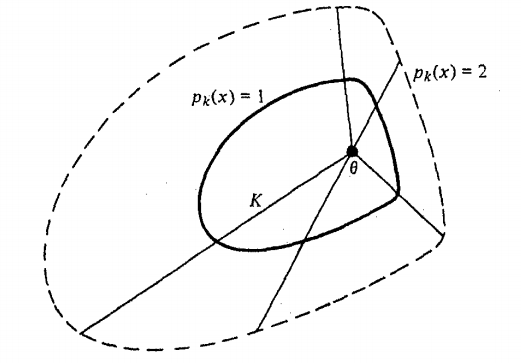
\includegraphics[scale = 0.5]{minkowski_functional_convex_set.png}}
\end{minipage}
\caption{\footnotesize{\textbf{The Minkowski functional of a convex set \citep{luenberger1997optimization}}}}
\label{fig: minkowski_functional_convex_set}
\end{figure}

\item \begin{lemma}
Let $K$ be a convex set containing $0$ as an interior point. Then \textbf{the Minkowski functional} $p$ of $K$ satisfies:
\begin{enumerate}
\item $0 \le p(x) < \infty$ for all $x \in X$;
\item (\textbf{Homogeneity}): $p(\lambda x) = \lambda p(x)$ for all $\lambda \ge 0$ and $x \in X$;
\item (\textbf{Sublinearity}): $p(x + y) \le p(x) + p(y)$,
\item $p$ is \textbf{continuous};
\item $\overline{K} = \{x: p(x) \le 1\}$ and $\mathring{K} = \{x : p(x) < 1\}$.
\end{enumerate}
\end{lemma}
That is, \emph{the Minkowski functional} is \emph{a sublinear functional}.

\item \begin{theorem} (\textbf{Mazur's Theorem, \underline{Geometric Hahn-Banach Theorem}}) \citep{luenberger1997optimization}\\
Let $K$ be a \underline{\textbf{convex set} having a \textbf{nonempty interior}} in a real normed linear vector space $X$. Suppose $V$ is a \textbf{linear variety} in $X$ \underline{containing no interior points} of $K$. Then there is a \underline{\textbf{closed hyperplane}} in $X$ \underline{containing $V$ but \textbf{containing no interior points} of $K$}; i.e., there is an element $f \in X^{*}$ and a constant $c$ such that $f(v) = c$ for all $v \in V$ and $f(k) < c$ for all $k \in K$.
\end{theorem}
\begin{proof}
By an appropriate translation we may assume that $0$ is an interior point of $K$. Let \emph{$M$ be the subspace of $X$ generated by $V$}. Then $V$ is a \emph{\textbf{hyperplane}} in $M$ and does not contain $0$; thus there is a \emph{\textbf{linear functional}} $f$ on $M$ such that $V = \{x :f(x) = 1\}$.

We then show that $f(x) \le p(x)$ for all $x \in M$, where $p(x)$ is \emph{\textbf{the Minkowski functional}} (a sublinear functional). Since $V$ contains no interior
point of $K$, we have $f(x) = 1 \le  p(x)$ for $x \in V$. By homogeneity, $f(\alpha x) = \alpha \le p(\alpha x)$ for $x \in V$ and $\alpha > 0$. While for $\alpha < 0$, $f(\alpha x) \le 0 \le p(\alpha x)$. Thus $f(x) \le p(x)$ for all $x \in M$.

Then by \emph{the Hahn-Banach Theorem}, there is an \emph{\textbf{extension}} $F$ of $f$ from $M$ to $X$ with $F(x) \le p(x)$. Let $H= \{x: F(x) = 1\}$. Since $F(x) \le p(x)$ on $X$ and since by Lemma 1 $p$ is \emph{\textbf{continuous}}, $F$ is \emph{\textbf{continuous}}, $F(x) < 1$ for $x \in \mathring{K}$, therefore, $H$ is the desired closed hyperplane. \qed
\end{proof}


\item \begin{remark} (\emph{\textbf{Geometric Interpretation of the Hahn-Banach theorem}})\\
\emph{The \textbf{geometric form} of the \textbf{Hahn-Banach theorem}}, in simplest form, says that given \emph{a \textbf{convex set}} $K$ containing \emph{\textbf{an interior point}}, and given a point $x_0$ \emph{not in} $\mathring{K}$, there is a \emph{\textbf{closed hyperplane}} \emph{\textbf{containing}} $x_0$ but \emph{\textbf{disjoint}} from $\mathring{K}$.
\end{remark}



\item \begin{definition} (\emph{\textbf{Supporting Hyperplane}})\\
A \emph{\textbf{closed} hyperplane} $H$ in a normed space $X$ is said to be \underline{\emph{\textbf{a supporting hyperplane}}} (or a  \emph{\textbf{support}}) for the \emph{\textbf{convex set}} $K$ if $K$ is \emph{contained} in \emph{one of the \textbf{closed half-spaces}} determined by $H$ and $H$ contains a point of $\overline{K}$.
\end{definition}

\begin{figure}
\begin{minipage}[t]{1\linewidth}
  \centering
  \centerline{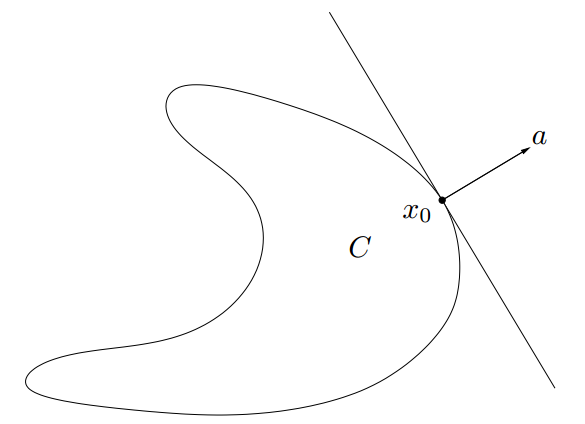
\includegraphics[scale = 0.4]{supporting_hyperplane.png}}
\end{minipage}
\caption{\footnotesize{\textbf{The supporting hyperplane of a convex set \citep{boyd2004convex}}}}
\label{fig: supporting_hyperplane}
\end{figure}

\item \begin{remark}
Suppose $K \subseteq \bR^n$, and $x_0$ is a point in its boundary $\partial K$, i.e.,
\begin{align*}
x_0 \in \partial K = \overline{K} \setminus \mathring{K}.
\end{align*}
If $a \neq 0$ satisfies $\inn{a}{x} \le  \inn{a}{x_0}$ for all $x \in K$, then the hyperplane $\{x: \inn{a}{x} = \inn{a}{x_0}\}$
is called \emph{\textbf{a supporting hyperplane}} to $K$ at the point $x_0$.
\end{remark}

\item \begin{theorem} (\underline{\textbf{Supporting Hyperplane Theorem}}) \citep{luenberger1997optimization, rockafellar1970convex} \\
If $x$ is \textbf{not an interior point} of a convex set $K$ which contains interior points, there is a \textbf{closed hyperplane} $H$ containing $x$ such that $K$ lies on one side of $H$.
\end{theorem}


\begin{figure}
\begin{minipage}[t]{1\linewidth}
  \centering
  \centerline{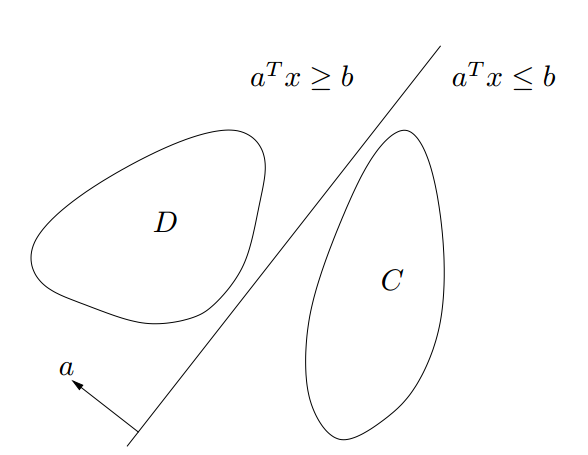
\includegraphics[scale = 0.4]{separating_hyperplane_theorem.png}}
\end{minipage}
\caption{\footnotesize{\textbf{The existence of a separating hyperplane between two convex sets that does not overlap in interior set. \citep{boyd2004convex}}}}
\label{fig: separating_hyperplane_theorem}
\end{figure}


\item As a consequence of the above theorem, it follows that, for a convex set $K$ with interior points, \emph{\textbf{a supporting hyperplane} can be constructed
containing \textbf{any boundary point of $\overline{K}$}}.
\begin{theorem} (\underline{\textbf{Eidelheit's Separation Theorem}})  \citep{luenberger1997optimization, rockafellar1970convex} \\
Let $K_1$ and $K_2$ be \textbf{convex sets} in $X$ such that $K_1$ has interior points and $K_2$ \textbf{contains no interior point of $K_1$}.
Then there is a \textbf{closed hyperplane} $H$ \textbf{separating} $K_1$ and $K_2$; i.e., there exists $f \in X^{*}$ such that 
\begin{align}
\sup_{x \in K_1}f(x) &\le \inf_{x \in K_2}f(x) \label{eqn: convex_duality_weak}
\end{align}
In other words, $K_1$ and $K_2$ lie in \textbf{opposite} \textbf{half-spaces} determined by $H$.
\end{theorem}
\begin{proof}
Let $K = K_1 - K_2 = \set{x_1 - x_2: x_1 \in K_1, x_2 \in K_2}$; then $K$ contains an interior point and $0$ not one of them. Also $K$ is a convex set. By \emph{The Supporting Hyperplane Theorem},  there is an $f \in X^{*}$, $f \neq 0$, such that $f(x) \le 0$ for $x \in K$. Thus for $x_1 \in K_l$, $x_2 \in K_2$, $f(x_1) \le f(x_2)$. Consequently, there is a real number $c$ such that $\sup_{x \in K_1}f(x) \le c \le \inf_{x \in K_2}f(x)$. The desired hyperplane is $H = \{x:  f(x) = c\}$.  \qed
\end{proof}

\item \begin{corollary}
If $K$ is a \textbf{closed convex} set and $x \not\in K$, there is a \textbf{closed halfspace} that contains $K$ but does not contain $x$.
\end{corollary}

\item \begin{theorem} (\textbf{Dual Representation of Convex Set})\citep{luenberger1997optimization, rockafellar1970convex} \\
If $K$ is a \textbf{closed convex} set in a normed space, then $K$ is equal to the \textbf{intersection} of all the \textbf{closed half-spaces} that contain it. 
\end{theorem}

\item \begin{remark} (\emph{\textbf{Duality for Convex Set}})\\
Theorem above is often regarded as \emph{\textbf{the geometric foundation} of \textbf{duality theory} for \textbf{convex sets}}. By associating \emph{closed hyperplanes} (or \textit{half-spaces}) with elements of $X^{*}$, the theorem expresses \emph{\textbf{a convex set in $X$ as a collection of elements in $X^{*}$}}. See more in \citep{rockafellar1970convex}.
\end{remark}

\item \begin{definition}
Let $K$ be a convex set in a real normed vector space $X$. The functional
\begin{align*}
h(f) &:= \sup_{x \in K}f(x)
\end{align*} defined on $X^{*}$ is called \underline{\emph{\textbf{the support functional}}} of $K$. $h \in X^{**}$.
\end{definition}

\item \begin{remark}
The \emph{\textbf{support functional}} of a \emph{convex set $K$} \emph{completely specifies the set (to within \textbf{closure})}
\begin{align*}
\overline{K} &= \bigcap_{f \in X^{*}}\set{x: f(x) \le h(f)}.
\end{align*}
\end{remark}

\end{itemize}

\section{Linear Operators in Banach Space}
\subsection{Adjoints of Bounded Operator}
\begin{itemize}
\item \begin{definition} (\emph{\textbf{Banach Space Adjoint}})\\
Let $X$ and $Y$ be \emph{Banach spaces},  $T$ \emph{a \textbf{bounded linear operator}} from $X$ to $Y$. The \underline{\emph{\textbf{Banach space adjoint of $T$}}}, denoted by $T^{'}$, is \emph{the \textbf{bounded linear operator} from $Y^{*}$ to $X^{*}$} defined by 
\begin{align*}
\paren{T'f}(x) &= f\paren{Tx}
\end{align*} for all $f \in Y^{*}$, $x \in X$. 
\end{definition}

\item \begin{example} (\emph{\textbf{Adjoint of Right Shift Operator}})\\
Let $X = \ell^1 = Y$ and let $Τ$ be \emph{\textbf{the right shift operator}}
\begin{align*}
T\paren{\xi_1, \xi_2, \ldots} &= \paren{0, \xi_1, \xi_2, \ldots}
\end{align*}
Then $T':  \ell^{\infty} \rightarrow \ell^{\infty}$ is \emph{\textbf{the left shift  operator}} 
\begin{align*}
T'\paren{\xi_1, \xi_2, \ldots} &= \paren{\xi_2, \xi_3, \ldots}.
\end{align*}
\end{example}

\item \begin{proposition} (\textbf{Isomorphism between Bounded Operator and its Adjoint}). \citep{reed1980methods}\\
Let $X$ and $Y$ be \textbf{Banach spaces}. The map $T \rightarrow T'$ is an \textbf{isometric isomorphism} of  $\cL(X, Y)$ into $\cL(Y^{*}, X^{*})$. 
\end{proposition}

\item \begin{remark} (\emph{\textbf{Hilbert Space Adjoint}})\\
Let $\cL(\cH):= \cL(\cH, \cH)$ be \emph{the space of bounded linear operators} on $\cH$. \emph{The Banach space adjoint} of $T^{*}$  then a mapping of  $\cH^{*}$ to $\cH^{*}$. Let $C:  \cH \rightarrow  \cH^{*}$ be the map which assigns to each $y \in \cH$, the bounded linear functional $\inn{y}{\cdot}$ in $\cH^{*}$.  $C$ is a \underline{\emph{\textbf{conjugate linear isometry}}} which is \emph{\textbf{surjective}} by \emph{the Riesz Representation theorem} (so it is \emph{\textbf{unitary}}). Now define a map $T^{*}: \cH \rightarrow \cH$ by 
\begin{align*}
T^{*} &= C^{-1}T' C
\end{align*}
Then $T^{*}$ satisfies 
\begin{align*}
\inn{x}{Ty} = (Cx)(Ty) = (T'Cx)(y) = \inn{C^{-1}T'Cx}{y} = \inn{T^{*}x}{y},
\end{align*}
$T^*$ is called  \underline{\emph{\textbf{the Hilbert space adjoint of $T$}}}, but usually we will just call it the  adjoint and let the $T^*$ distinguish it from $T'$. Notice that the map $T \rightarrow T^*$ is \emph{\textbf{conjugate linear}}, that is, $\alpha T  \rightarrow \bar{\alpha} T^*$. This is because $C$ is conjugate linear. 
\end{remark}

\item \begin{proposition} \citep{reed1980methods}\\
The map $T \rightarrow T^*$ is always \textbf{continuous} in the \textbf{weak} and \textbf{uniform operator topologies} but is only continuous in the \textbf{strong operator topology} if $\cH$ is \textbf{finite dimensional}. 
\end{proposition}
\end{itemize}

\subsection{Baire Category Theorem}
\begin{itemize}
\item \begin{remark} (\emph{\textbf{Empty Interior $=$ Complement is Dense}}) \\
Recall that if $A$ is a subset of a space $X$, the \emph{\textbf{interior}} of $A$ is defined as \emph{the union of all open sets of $X$ that are contained in $A$}. 

To say that $A$ has \underline{\emph{\textbf{empty interior}}} is to say then that \emph{\textbf{$A$ \underline{contains no open set} of $X$} other than the empty set}. \emph{\textbf{Equivalently}}, $A$ has \emph{\textbf{empty interior}} if every point of $A$ is \emph{a \textbf{limit point} of the \textbf{complement} of $A$}, that is, if \underline{\emph{the \textbf{complement} of $A$ is \textbf{dense} in $X$}}.
\begin{align*}
\mathring{A} = \emptyset \;\; \Leftrightarrow \;\; A^{c}\text{ is dense in }X
\end{align*} In \citep{reed1980methods}, if a subset $\overline{A}$ of $X$ has \emph{empty interior}, $A$ is said to be \underline{\emph{\textbf{nowhere dense}}} in $X$.
\end{remark}

\item \begin{example} 
Some  examples:
\begin{enumerate}
\item The set $\bQ$ of \emph{rationals} has \emph{\textbf{empty interior}} as a subset of $\bR$
\item The \emph{interval} $[0, 1]$ has \emph{\textbf{nonempty interior}}. 
\item The \emph{interval} $[0, 1] \times 0$ has \emph{\textbf{empty interior}} as a \emph{subset of the plane} $\bR^2$, and so does the \emph{subset} $\bQ \times \bR$.
\end{enumerate}
\end{example}

\item \begin{definition} (\emph{\textbf{Baire Space}})\\
A space $X$ is said to be a \underline{\emph{\textbf{Baire space}}} if the following condition holds:  Given  \emph{\textbf{any countable}} collection $\set{A_n}$ of \emph{\textbf{closed}} sets of $X$ each of which has \emph{\textbf{empty interior}} in $X$, their \emph{\textbf{union}}  $\bigcup_{n=1}^{\infty} A_n$ also has \emph{\textbf{empty interior}} in $X$.
\end{definition}

\item \begin{example} 
Some  examples:
\begin{enumerate}
\item The space $\bQ$ of \emph{rationals} is \emph{\textbf{not} a \textbf{Baire space}}. For each one-point set in $\bQ$ is \emph{closed and has empty interior \textbf{in $\bQ$}}; and $\bQ$ is \emph{the countable union of its one-point subsets}.
\item The space $\bZ_{+}$, on the other hand, does form \emph{a \textbf{Baire space}}. Every subset of $\bZ_{+}$ is \emph{open}, so that there exist \emph{no subsets} of $\bZ_{+}$ having \emph{empty interior}, except for the empty set. Therefore, $\bZ_{+}$ satisfies the Baire condition vacuously.
\item The \emph{interval} $[0, 1] \times 0$ has \emph{\textbf{empty interior}} as a \emph{subset of the plane} $\bR^2$, and so does the \emph{subset} $\bQ \times \bR$.
\end{enumerate}
\end{example}

\item \begin{definition}  (\emph{\textbf{Baire Category}})\\
A subset $A$ of a space $X$ was said to be of \underline{\emph{\textbf{the first category in $X$}}} if it \emph{\textbf{was contained} in the \textbf{union} of a \textbf{countable} collection of \textbf{closed} sets of $X$ having \textbf{empty interiors} in $X$}; \emph{\textbf{otherwise}}, it was said to be of \underline{\emph{\textbf{the second category in $X$}}}. 
\end{definition}

\item \begin{remark}
\emph{A space $X$ is a \textbf{Baire space} if and only if every \textbf{nonempty open} set in $X$ is of \textbf{the second category}}.
\end{remark}

\item \begin{lemma}(\textbf{Open Set Definition of Baire Space}) \citep{munkres2000topology} \\
$X$ is a \textbf{Baire space} \textbf{if and only if} given any \textbf{countable} collection $\set{U_n}$ of \textbf{open} sets in $X$, each of which is \textbf{dense} in $X$, their \textbf{intersection} $\bigcap_{n=1}^{\infty}U_n$ is also \textbf{dense} in $X$.
\end{lemma}

\item \begin{theorem} (\textbf{Baire Category Theorem}).  \citep{munkres2000topology} \\
If $X$ is a \textbf{compact Hausdorff} space or a \textbf{complete metric space}, then $X$ is a \textbf{Baire space}.
\end{theorem}

\item \begin{remark}
In other word,  neither \textbf{\emph{compact Hausdorff}} space or a \textbf{\emph{complete metric space}} is a \emph{countable union of closed subsets with empty interior (that are nowhere dense)}.
\end{remark}

\item \begin{lemma}\citep{munkres2000topology} \\
Let $C_1 \supset C_2 \supset \ldots$ be a \textbf{nested} sequence of \textbf{nonempty closed sets} in the \textbf{complete metric space} $X$. If $\text{diam }C_n \rightarrow 0$, then $\bigcap_{n}C_n  = \emptyset$.
\end{lemma}

\item \begin{lemma} \citep{munkres2000topology} \\
Any \textbf{open} subspace $Y$ of a Baire space $X$ is itself a Baire space.
\end{lemma}

\item \begin{theorem} (\textbf{Discontinuity Point of Pointwise Convergence Function}) \citep{munkres2000topology} \\
Let $X$ be a space; let $(Y, d)$ be a metric space. Let $f_n : X \rightarrow Y$ be a sequence of continuous functions such that $f_n(x) \rightarrow f(x)$ for all $x \in X$, where $f : X \rightarrow Y$. If $X$ is a \textbf{Baire space}, the set of points at which $f$ is \textbf{continuous} is \textbf{dense} in $X$.
\end{theorem}

\item \begin{remark} (\textbf{\emph{Use Baire Category Theorem as Proof by Contradition}})\\
\emph{\textbf{The Baire category theorem}} is used to prove a certain subset $C$ is \emph{\textbf{dense}} in $X$ by stating that $X$ is a Baire space and $C$ is countable intersection of dense open subsets in $X$ (\emph{$C$ is a $G_{\delta}$ sets}). 

On the other hand, if $M =  \bigcup_{n=1}^{\infty}A_n$ has \emph{\textbf{nonempty interior}}, then \emph{\textbf{some}} of the  sets $\bar{A}_n$ \emph{\textbf{must have nonempty interior}}. Otherwise, it contradicts with the Baire space definition.
\end{remark}
\end{itemize}

\subsection{Uniform Boundedness Theorem}
\begin{itemize}
\item \begin{proposition}\label{prop: bounded_non_empty_int} \citep{reed1980methods}\\
Let $X$ and $Y$ be normed linear spaces. Then a linear map  $Τ: X\rightarrow Y$ is \textbf{bounded} if and only if 
\begin{align*}
T^{-1}\set{y: \norm{y}{Y} \le 1}
\end{align*} has a \textbf{nonempty interior}. 
\end{proposition}
\begin{proof}
Suppose that $T$ is given and the set in question contains the ball
\begin{align*}
\set{x:  \norm{x - x_0}{X} < \epsilon} 
\end{align*}
Then $\norm{x}{} < \epsilon$ implies  $x + x_0$ is in the ball of radius $\epsilon$ about $x_0$. Thus $\norm{T (x + x_0)}{Y} \le 1$ and 
\begin{align*}
\norm{T x}{Y} \le  \norm{T (x + x_0)}{Y} + \norm{T(x_0)}{Y} \le  1 + \norm{T(x_0)}{Y}.
\end{align*}
Thus for \emph{all} $x \in X$, 
\begin{align*}
\norm{T x}{Y} \le  \epsilon^{-1}\paren{1 + \norm{T(x_0)}{Y}}\norm{x}{X} 
\end{align*}
so $Τ$ is \emph{bounded}. The \emph{converse} is easy. \qed
\end{proof}

\item \begin{theorem} (\textbf{The Uniform Boundedness Theorem}). \citep{reed1980methods} \\
Let $X$ be a \textbf{Banach space}. Let $\srF$ be a family of \textbf{bounded} linear transformations from $X$ to some \textbf{normed linear space} $Y$. Suppose that for each $x \in X$, $\set{\norm{Tx}{Y}:  T \in \srF}$ is  \textbf{bounded}, i.e.
\begin{align*}
\sup_{T \in \srF}\norm{Tx}{Y} < \infty.
\end{align*} Then $\set{\norm{T}{}: T \in \srF}$ is \textbf{bounded}, i.e.
\begin{align*}
\sup_{T \in \srF}\norm{T}{} < \infty.
\end{align*}
\end{theorem}
\begin{proof}
Let 
\begin{align*}
B_n := \set{x: \norm{Tx}{Y} \le n, \;\forall \, T \in \srF}.
\end{align*} By the hypothesis each $x$ is in some $B_n$, that is, $X = \bigcup_{n=1}^{\infty}B_n$.  Moreover each $B_n$ is \textbf{\emph{closed}} since each $T$ is  continuous. By \emph{the Baire category theorem}, some $B_n$ has a \emph{\textbf{nonempty interior}}. By proposition \ref{prop: bounded_non_empty_int}, we conclude that the $\norm{T}{}$'s are \emph{uniformly bounded}. \qed
\end{proof}

\item \begin{corollary} (\textbf{Separately Continuity of Bilinear Form on Banach Space $=$ Joint Continuity}) \citep{reed1980methods}\\
Let $X$ and $Y$ be Banach spaces and let $B(\cdot,  \cdot)$ be a \textbf{separately continuous bilinear mapping} from $X \times Y$ to $\bC$, that is, it is a \textbf{bounded} linear transformation if one of the two arguments is fixed. Then $B(\cdot,  \cdot)$ is \textbf{jointly continuous}, that is, if $x_n \rightarrow 0$ and  $y_n \rightarrow 0$ then $B(x_n, y_n) \rightarrow 0$. 
\end{corollary}
\end{itemize}

\subsection{Open Mapping Theorem}
\begin{itemize}
\item 
\begin{theorem} (\textbf{Open Mapping Theorem}) \citep{reed1980methods} \\
Let $T: X \rightarrow Y$ be a \textbf{\underline{surjective} bounded linear transformation} of one \textbf{Banach} space \underline{\textbf{onto}} another \textbf{Banach} space $Y$.  Then if $M$ is an \textbf{open} set in $X$, $T(M)$ is \textbf{open} in $Y$. 
\end{theorem}
\begin{proof}
We need  only show that, for every \emph{neighborhood} $N$ of $x$, $T(N)$ is a \emph{neighborhood} of  $T(x)$. Since $T(x + N) = T(x) + T(N)$, we need only show this for $x = 0$.  Since neighborhoods contain balls it is sufficient to show that $T(B_{X}(0,r)) \supseteq B_{Y}(0, r')$, for 
some $r'$ where 
\begin{align*}
B_{X}(0, r) &= \set{x \in X: \norm{x}{X} < r}.
\end{align*}
However, since $T(B_{X}(0,r)) = r\,T(B_{X}(0,1))$, we need only show that $T(B_{X}(0,r))$ is a \emph{neighborhood} of \emph{zero} for some $r$. Finally, by the ``\emph{translation argument}" of the proposition, it is sufficient to show that $T(B_{X}(0,r))$ has a \emph{\textbf{nonempty interior}} for  \emph{\textbf{some}} $r$. 

Since $T$ is \emph{\textbf{onto}}, 
\begin{align*}
Y &= \bigcup_{n=1}^{\infty}T(B_{X}(0, n))
\end{align*}
so some $\overline{T(B_{X}(0, n))}$ has a \emph{\textbf{nonempty interior}}. 

Now the hard work begins, since we want $T(B_{X}(0, n))$ to have a \emph{nonempty interior}. By scaling and translating, we can 
suppose that $B_{Y}(0, \epsilon)$ is contained in $\overline{T(B_{X}(0, 1))}$; we will show that $\overline{T(B_{X}(0, 1))} \subset T(B_{X}(0, 2))$ 
which will complete the proof. 

Let $y\in \overline{T(B_{X}(0, 1))}$. Pick $x_1 \in B_{X}(0,1)$ so $y - Tx_1 \in B_{Y}(0, \epsilon/2) \subset \overline{B_Y(0, 1/2)}$. Now pick $x_2 \in B_{X}(0,1/2)$ 
so that 
\begin{align*}
y - Tx_1 -Tx_2 \in B_{Y}(0, \epsilon/4)
\end{align*}
By induction, we choose $x_n \in B_{X}(0, 2^{1-n})$ so that 
\begin{align*}
y - \sum_{j=1}^n T x_j \in B_{Y}(0, 2^{1-n}\epsilon)
\end{align*}
Then $x = \sum_{j=1}^{\infty}x_j$ \emph{exists} and is in $B_X(0, 2)$ and 
\begin{align*}
y = \sum_{j=1}^{\infty} T x_j = Tx.
\end{align*}
Thus $y \in T(B_{X}(0, 2))$. \qed
\end{proof}

\item \begin{corollary} (\textbf{Inverse Mapping Theorem}) \citep{reed1980methods} \\
A \textbf{continuous} \textbf{bijection} of one Banach space onto another has a \textbf{continuous} \textbf{inverse}. 
\end{corollary}

\item \begin{remark}
Note $T$ is an open map and $A = T^{-1}(T(A))$ for surjective map, then $T^{-1}$ is \emph{continuous}.
\end{remark}

\item \begin{theorem} (\textbf{Banach-Schauder Theorem}) \citep{reed1980methods}\\
Let $T$ be a \textbf{continuous} linear map, $T: E \rightarrow F$,  where $E$ and $F$ are Banach spaces. Then either $T(A)$ is \textbf{open} in $T(E)$  for \textbf{each open} $A \subseteq E$,  or $T(E)$  is of \textbf{first category} in $\overline{T(E)}$.
\end{theorem}
\end{itemize}

\subsection{Closed Graph Theorem}
\begin{itemize}
\item \begin{definition} (\emph{\textbf{Graph of Function}})\\
Let $Τ$ be a mapping of a normed linear space X into a normed  linear space Y. The \underline{\emph{\textbf{graph of $T$}}}, denoted by $\Gamma(T)$, is defined as 
\begin{align*}
\Gamma(T) := \set{(x,y) \in X \times Y: y = Tx}.
\end{align*}
\end{definition}


\item \begin{theorem} (\textbf{Closed Graph Theorem})\citep{reed1980methods} \\
Let $X$ and $Y$ be Banach spaces  and $T$ a linear map of $X$ into $Y$. Then $T$ is \textbf{bounded} if and only if the \textbf{graph} of 
$Τ$ is \textbf{closed}. 
\end{theorem}
\begin{proof}
Suppose that $\Gamma(T)$ is \emph{\textbf{closed}}. Then, since $Τ$ is linear, $\Gamma(T)$ is a \emph{\textbf{subspace}}  of \emph{\textbf{the Banach space direct sum}} $X \oplus Y$. By assumption $\Gamma(T)$ is \emph{\textbf{closed}} and thus is a \emph{\textbf{Banach space}} in the norm 
\begin{align*}
\norm{(x, Tx)}{} &= \norm{x}{X} + \norm{Tx}{Y}
\end{align*}
Consider the \emph{\textbf{continuous} projection maps} $\pi_1$ and $\pi_2$, 
\begin{align*}
\pi_1: (x, Tx) \mapsto x, \quad \pi_2: (x, Tx) \mapsto Tx.
\end{align*}
$\pi_1$ is a \emph{\textbf{bijection}} so by \emph{\textbf{the inverse mapping theorem}} $\pi_1^{-1}$ is \emph{\textbf{continuous}}. But 
$T = \pi_2 \circ \pi_1^{-1}$, so $T$ is \emph{\textbf{continuous}}. The \emph{converse} is \emph{trivial}. \qed 
\end{proof}

\item \begin{remark}
To avoid future confusion, we emphasize that the $T$ in this theorem is implicitly assumed to be \emph{\textbf{defined on all of $X$}}. 
\end{remark}

\item \begin{remark}
Consider the following statements: 
\begin{enumerate}
\item $x_n$ converges to some element $x$;
\item $T x_n$ converges to some element $y$; 
\item $T x_n = y$.
\end{enumerate} 
Usually to prove $T$ is continuous, one need to show that given statement $1$, the statement $2$ and $3$ are true. That is, we need to \emph{\textbf{prove convergence}} of $T x_n$ and need to show \emph{\textbf{identification}} of $T x$ and the limit of $T x_n$.

With \emph{\textbf{close graph theorem}}, we just need to show that given statement $1$ \emph{\textbf{and}} $2$, statement $3$ is true; that is, we just need to prove the identification part.
\end{remark}

\item \begin{corollary}(\textbf{The Hellinger-Toeplitz Theorem}) \citep{reed1980methods} \\
Let $A$ be an \textbf{everywhere defined} linear operator on a \textbf{Hilbert space} $\cH$ with
\begin{align*}
\inn{x}{Ay} &= \inn{Ax}{y}
\end{align*} for all $x, y \in \cH$; that is $A$ is \textbf{self-adjoint}. Then $A$ is \textbf{bounded}. 
\begin{proof}
We will prove that $\Gamma(A)$ is \textbf{closed}. Suppose that $\inn{x_n}{Ax_n} \rightarrow \inn{x}{y}$. 
We need only prove that $\inn{x}{y} \in \Gamma(A)$, that is, that $y = Ax$. For any $z \in \cH$,
\begin{align*}
\inn{z}{y} &= \lim\limits_{n \rightarrow \infty}\inn{z}{Ax_n} = \lim\limits_{n \rightarrow \infty}\inn{Az}{x_n}\\
&= \inn{Az}{x} = \inn{z}{Ax}
\end{align*}
Thus $y = Ax$ and $\Gamma(A)$ is \textbf{closed}. \qed
\end{proof}
\end{corollary}
\end{itemize}

\newpage
\bibliographystyle{plainnat}
\bibliography{reference.bib}
\end{document}